\section{Piezoelektrizität}
%% TODO: improve this paragraph
Die Piezoelektrizität ist die spannende Eigenschaft, dass gewisse Kristalle eine elektrische Spannung erzeugen, wenn mechanischer Druck auf sie ausgeübt wird.

\begin{figure}
    \centering
    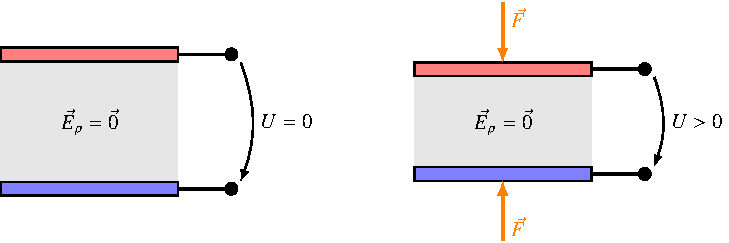
\includegraphics[]{papers/punktgruppen/figures/piezo} %das Efeld mit Naoki disskutieren, müssen sicher gehen, dass es mit jenen in Abbildung Piezo aufbau übereinstimmt
    \caption{Piezoelektrisches Material in Ruhe und unter Druck}
    \label{fig:punktgruppen:basicPiezo}
\end{figure}

\subsection{Polarisierung}
Piezoelektrizität basiert darauf, dass zwischen den Oberflächen des Kristalles ein Ladungsungleichgewicht entsteht (siehe Abbildung\ref{fig:punktgruppen:basicPiezo}).
Dieses Ungleichgewicht resultiert, 
weil durch den mechanischen Druck auf der einen Oberfläche des Kristalles positive Ionen näher an die Oberfläche gelangen,
wärend auf der gegenüberliegenden Seite dasselbe mit negativen Ionen passiert.
Es besitzt jedoch nicht jeder Kristall eine atomare Struktur welche sich unter Druck genau so verformt.
Der Aufbau und somit auch die Symmetrie des Kristalles sind daher relevant für die Entstehung dieses Effektes.

\begin{figure}
    \centering
    \begin{tabular}{c |c}
      \subfigure[][\label{fig:punktgruppen:atoms-piezo}]{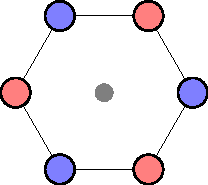
\includegraphics{papers/punktgruppen/figures/atoms-piezo-still}} &
      \subfigure[][\label{fig:punktgruppen:atoms-grid}]{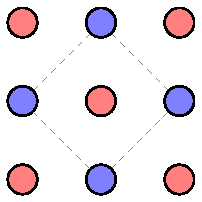
\includegraphics{papers/punktgruppen/figures/atoms-grid-still}} \\
      \subfigure[][\label{fig:punktgruppen:atoms-piezo-fv}]{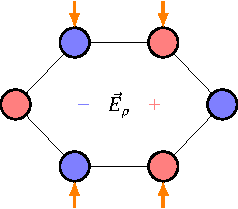
\includegraphics{papers/punktgruppen/figures/atoms-piezo-force-vertical}}
      \hspace{2mm}
      \subfigure[][\label{fig:punktgruppen:atoms-piezo-fh}]{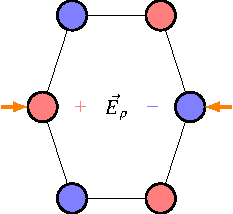
\includegraphics{papers/punktgruppen/figures/atoms-piezo-force-horizontal}}
      \hspace{3mm} & \hspace{3mm}
      \subfigure[][\label{fig:punktgruppen:atoms-grid-f}]{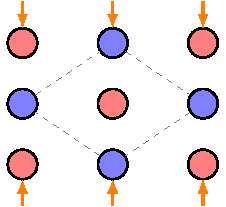
\includegraphics{papers/punktgruppen/figures/atoms-grid-force}} \\
    \end{tabular}
    \caption{
        Kristallstrukturen mit und ohne piezoelektrischer Eigenschaft.
    }
    \label{fig:punktgruppen:atomPiezo}
\end{figure}

\subsection{Atomarer Aufbau}
Die Polarisation entsteht an der Oberfläche eines Kristalles, die Erklärung dazu finden wir jedoch im atomaren Aufbau.
Wir wollen dazu die verschiedenen Kristallstrukturen auf Abbildung \ref{fig:punktgruppen:atomPiezo} diskutieren.
In Abbildung \ref{fig:punktgruppen:atomPiezo} gilt für alle Strukturen, dass rote Kreise positive Ionen und blaue negative Ionen repräsentieren. 
Struktur \subref{fig:punktgruppen:atoms-piezo} zeigt ein piezoelektrisches Material in Ruhe. 
Struktur \subref{fig:punktgruppen:atoms-piezo-fv} ist dasselbe Kristallgitter, jedoch wird es senkrecht belastet. 
Eingezeichnet ist auch das elektrische Feld, welches entsteht, weil die Ladungsträger ganz links und rechts weiter auseinander gedrückt werden.
Als Hilfe zur Vorstellung kann man \subref{fig:punktgruppen:atoms-piezo-fv} zwischen zwei leitende Platten setzen, so wird ersichtlich, 
dass mit wachsendem Druck eine negative Ladung an die rechte Platte gedrückt wird, während sich die positiven Ionen weiter entfernen. 
\par
Die Struktur \subref{fig:punktgruppen:atoms-grid} ist nicht piezoelektrisch.
Dies wird ersichtlich, wenn man \subref{fig:punktgruppen:atoms-grid} unter Druck setzt und sich die Struktur zu \subref{fig:punktgruppen:atoms-grid-f} verformt.
Setzt man \subref{fig:punktgruppen:atoms-grid-f} gedanklich auch zwischen zwei leitende Platten, 
scheint es als würden rechts mehr positive Ionen in die Platte gedrückt werden und links umgekehrt.
Dies ist aber nicht mehr der Fall, wenn sich die Struktur nach oben und unten periodisch wiederholt.
\par
Struktur \subref{fig:punktgruppen:atoms-piezo-fh} zeigt \subref{fig:punktgruppen:atoms-piezo} in unter horizontaler Belastung. 
Was zwischen \subref{fig:punktgruppen:atoms-piezo-fv} und \subref{fig:punktgruppen:atoms-piezo-fh} zu beobachten ist, 
ist, dass die entstandene Ladungsdifferenz orthogonal zu der angelegten Kraft entsteht, 
im Gegensatz zu \subref{fig:punktgruppen:atoms-piezo-fh}.
Daraus kann man schliessen, dass \subref{fig:punktgruppen:atoms-piezo} keine Rotationssymmetrie von \(90^\circ\) besitzen kann, 
weil die Eigenschaften der Struktur sich bei einer \(90^\circ\) Drehung ändern. 
Das Fehlen dieser Rotationssymmetrie bestätigt sich auch wenn \subref{fig:punktgruppen:atoms-piezo} als Hexagon betrachtet wird. 

\subsection{Punktsymmetrie}
Piezoelektrische Kristalle können nicht punktsymmetrisch sein.
Kristallgitter, bei welchen eine Punktspiegelung eine symmetrische Operation ist, können keine piezoelektrische Kristalle bilden.
Auf Abbildung \ref{fig:punktgruppen:atomPiezo} ist bewusst \subref{fig:punktgruppen:atoms-piezo} ein nicht punktsymmetrischer Kristall 
mit einem punktsymmetrischen \subref{fig:punktgruppen:atoms-grid} verglichen worden.
Als vereinfachte Erklärung kann man sich wieder das Bild eines Kristalles wie \subref{fig:punktgruppen:atoms-piezo} vor Augen führen, 
welcher unter Druck auf der einen Seite negative und der anderen Seite positive Ionen an seine Oberfläche verdrängt.
Spiegelt man nun den Kristall um den Gitterpunkt in der Mitte des Kristalles, so würden die negativen Ionen auf den positiven auf der anderen Seite landen,
was der Definition einer Symmetrie deutlich widerspricht.

\subsection{Vom Kristall zum Feuer}
Piezoelektrizität hat durchaus Nutzen im Alltag.
Feuerzeuge welche nicht auf dem Prinzip beruhen einen Zündstein abzuschleifen, 
sonder ohne Verschleiss auf Knopfdruck einen Zündfunken erzeugen, basieren auf dem Prinzip der Piezoelektrizität.
Drückt der Nutzende auf den Zündknopf, spannt sich eine Feder bis zu einer konfigurierten Spannung.
Wird vom Nutzenden fester zugedrückt entspannt sich die Feder schlagartig und beschleunigt mit der gespeicherten Energie ein Hammer,
welcher auf das Piezoelement aufschlägt.
Der augenblicklich hohe Druck sorgt an den Piezokontakten für eine eben so kurze aber hohe elektrische Spannung.
Die Spannung reicht aus, um eine Funkenstrecke zu überwinden und so eine entflammbares Gas zu entzünden.
Sollte der Leser eines Tages in die Situation geraten, in welcher er zwei verschiedene Kristalle vor sich hat und ein piezoelektrisches Feuerzeug bauen musst, wobei bekannt ist, dass der eine eine Punktsymmetrie aufweist, empfiehlt es sich, sich am anderen zu versuchen.

